% 제7회 한국 인공지능 학술대회 (KICS 인공지능소사이어티) 투고 원고
% 양식: manuscript/양식-논문샘플워드.doc 대응 (국문제목→저자→소속→이메일→영문제목→
%       영문저자→영문소속→요약→Ⅰ.서론…→참고문헌, 본문 2단, 최대 2쪽)
% 컴파일: Overleaf에서 XeLaTeX 선택 (kotex 한글)
\documentclass[a4paper,twocolumn,9pt]{extarticle}
\usepackage{kotex}\XeTeXlinebreaklocale ""
\usepackage[margin=2.0cm,top=2.5cm,bottom=2.5cm]{geometry}
\usepackage{graphicx}
\usepackage{amsmath}
\usepackage{setspace}
\usepackage[font=small,skip=3pt]{caption}
\usepackage{xcolor}
% 이번 개정에서 새로 쓰거나 고친 부분 표시 — 제출 전 \newcommand{\new}[1]{#1} 로 바꾸면 사라짐
\newcommand{\new}[1]{\textcolor{red}{#1}}
\setlength{\columnsep}{0.8cm}
\pagestyle{empty}

% 절 번호 로마숫자 (양식: Ⅰ. 서 론)
\renewcommand{\thesection}{\Roman{section}}
\makeatletter
\renewcommand\section{\@startsection{section}{1}{\z@}%
  {1.2ex plus .5ex}{0.8ex plus .3ex}{\centering\normalsize\bfseries}}
\makeatother

\begin{document}

% ===== 머리 블록 (1단 폭) =====
\twocolumn[{
\begin{center}
{\large\bfseries \new{VLA 내부 활성화로부터의 행동 단계 판독}}\\[1.2ex]
{박경태, 김상우, 오윤선$^{\dagger}$}\\
{한양대학교}\\[0.6ex] 
{\small rudxo1997@hanyang.ac.kr, $^{\dagger}$교신저자 이메일}\\[2.0ex] % TODO: 저자 이메일
{\large\bfseries \new{Reading the Current Action Phase\\ from the Internal Activations of a VLA Model}}\\[1.2ex]
{Kyungtae Park, Sangwoo Kim, Yoonseon Oh$^{\dagger}$}\\ 
{Hanyang Univ.}\\[2.0ex]
{\bfseries 요 약}
\end{center}
\begin{quote}\small
Vision-Language-Action(VLA) 모델이 작업을 수행할 때 스스로 현재 어떤 작업 단계를 진행중인지를 우리가 알 수 있다면, 이는 VLA모델에 대한 설명가능성과 추론 시 제어 및 개입의 출발점이 된다. 본 연구는 VLA의 내부 activation을 통해 모델이 스스로 인식하는 현재 작업 단계를 직접 읽는다. Gr00t N1.5의 action head(DiT)의 residual stream activation을 라벨 없이 clustering하면, \new{각 cluster는 특정 primitive action phase에 국한되어 나타나고 다른 phase에서는 잘 나타나지 않는다. 이 대응을 이용하면 한 번도 보지 않은 scene에서도 activation 한 스텝만으로 현재 phase를 정확도 0.86(비지도 clustering)/0.89(지도 probe)로 읽을 수 있으며, 이는 activation을 보지 않고 에피소드 진행 시간만 쓰는 대조군(0.61)을 크게 웃돈다. cluster는 사람이 정의한 phase보다 잘게 나뉘지만, 각 조각이 phase에 대해 순수하기 때문에 판독이 성립한다.} 이 구조는 데이터 처리 과정을 바꾸어도(AE$\rightarrow$SAE) 같은 시점에서 phase전환을 유지하고, 다양한 task,scene에서도 유지된다(z +8.8$\sim$+13.5). 즉, \new{VLA activation에는 action phase와 정합적인 구조가 존재해 추론 중 online 판독이 가능하며, 본 논문에서 이를 held-out 평가로 확인하였다.}
\end{quote}
\vspace{1.5ex}
}]

\begin{figure*}[!t]
  \centering
  
\includegraphics[width=0.96\textwidth]{figs/fig1_purity_residual.pdf}
  \caption{(a) 군집$\times$GT 단계 contingency(PPCC candle, k=8): 행을 최빈 단계로
  정렬하면 블록-대각 구조 --- 각 군집이 특정 phase에 국한된다(순도 0.888). (b) scene
  잔차화 후에도 phase margin은 유지되고(10/10 양수) (c) scene MI는 크게 준다.}
  \label{fig:purity}
\end{figure*}
\begin{figure}[!t]
  \centering
  
\includegraphics[width=\columnwidth]{figs/fig2_granularity_margin.pdf}
  \caption{(a) 발견 상태의 구간 길이는 GT 단계의 약 1/4$\sim$1/3. (b) 시간 대조군 대비
  MI margin: 고정 k KMeans가 자율 k 방식보다 높다(데이터셋 A, k=24 기준 +1.665
  bits).}
  \label{fig:granularity}
\end{figure}
\section{서 론}
많은 AI모델들이 그러하든 VLA 모델 또한 내부적으로 어떤 상태를 가지는지는 사람이 이해하기 힘든 블랙박스와 같다.  하지만 VLA모델은 실제 존재하는 로봇을 조작하기 때문에 LLM등과 달리 안전과 신뢰가 더욱 중요하다. 따라서 모델이 지금 무슨 작업을 진행중이라고 인지하는지 사람이 파악할 수 있어야 한다는 설명가능성(XAI)이 중요하다. 일반적으로 Pick \& Place task에서는 reach $\rightarrow$ grasp $\rightarrow$ transport $\rightarrow$ place 같은 primitive action phase를 사용할 수 있다. 이러한 현재 action phase를 파악하는 방법에는 외부 관찰자가 카메라나 기타 센서들을 활용해 로봇의 현재 상태나 궤적같은 외부 관찰자를 활용하는 방법이 있다. 하지만 이러한 외부 관찰자로는 현재 로봇이 보기에 무엇을 하고 있는지를 알려줄 뿐, 현재 저 로봇을 움직이는 인공지능이 스스로 무슨 action을 진행중인지는 알려주지 않는다. 모델이 스스로 무엇을 하고 있다고 인지하는지, 즉 모델의 internal representation이 가리키는 action phase는 모델 내부의 activation을 직접 읽어야만 알 수 있다. 이런 내부 표상을 아는것은 겉보기 행동과 어긋났을 경우에 수정을 진행 하기위한 전제 조건이다. VLA 내부 표현을 해석하려는 최근 시도들은
Sparse Auto Encoder(SAE)로 residual stream에서 grasp·transport 같은 primitive action에 대응하는 feature를 찾아내거나, linear probe로 layer별 상태를 관측하고 그 방향으로 activation steering을 적용해 행동을 제어 할 수 있음을 보였다. 그러나 이들은 사람이 rollout 영상을 검토해 발견 한 feature와 정렬해주어 이름을 붙힐 뿐, interval representation이 사람이 정의한 action phase와 어떤 해상도로 대응하는지 정량화하지 않는다. VLA의 internal action phase를 추론중에 online으로 읽을 수 있으면 설명을 넘어 조건부 개입이나 실패감지의 조건신호로 활용 할 수 있다. 본연구는 Gr00t N1.5가 RoboCasa환경에서 주방 조작을 수행하는동안 activation을 Autoencoder와 clustering을 사용해 분석하고 모델의 internal action phase가 사람이 붙힌 action phase와 어떤 관계를 가지는지를 MI를 활용해 정량화 한다. 

\section{방 법}
\textbf{Data} RoboCasa 주방 조작 환경에서 GR00T N1.5의 rollout을 수집한다.
대상은 5개 task(OpenDrawer, PnPCounterToCab, OvenRack, DishwasherRack,
CoffeeSetupMug)에 속하는 10개 instruction -- 같은 task로 분류되더라도 실제 모델에 들어가는 language instruction이 다른 case가 있으며, 분석은 이 instruction 단위로 수행한다-- 각instruction별로 10 scene에서, scene별로 diffusion noise를 다르게 해 10회 반복하여 데이터를 수집하였다. 각 rollout의 매 스텝에서 action head(DiT)의 residual stream activation을 캡처한다(layer 12, denoising step 3(last), 49개 토큰 평균 → 스텝당 1536차원). 여기서 한 \textbf{스텝}은 정책 추론 1회를 뜻하며 환경 5 스텝에 해당한다 --- 정책이 action chunk를 예측해 앞의 5개만 실행하고 다시 추론하므로, activation과 GT phase 라벨을 모두 이 시점에서 읽는다. 사람이 주석한 primitive action phase 라벨(instruction당 3~6단계)은 학습에 쓰지 않고 평가에만 사용한다. Detctor 학습에 사용된 데이터 % 학습에 몇개 추론에 몇개 어떻게 썼는지는 추후 작성

\textbf{Clustering.} raw activation(1536차원)을 그대로 오토인코더(AE, latent 16)로 압축한 뒤 KMeans로 스텝 단위 clustering한다(instruction별 분석은 k=8, 전체 통합 분석은 k=24). Cluster center는 train split에서만 만들고 평가 split의 스텝은 k-NN(k=15)으로 분류한다. 재군집화가 필요 없으므로 추론 중 스텝 단위 online 판독이 가능하다.

\textbf{Baseline.} Activation이 action phase 정보를 담는지 재려면, 먼저 ``진행 시간만 알아도 맞힐 수 있는 몫''을 빼야 한다. Manipulation task의 action phase는 대체로 순서대로 진행되므로 activation을 전혀 보지 않고 경과 시간만 보는 판독기도 phase의 정. 이를 \textbf{시간 대조군}으로 정의한다: 에피소드 내 상대 진행도 $t/T$를 발견된 군집
수와 같은 개수의 구간으로 등분위 분할해 얻은 상태열이다. 상태 수를 맞추는 이유는 상태
수가 많을수록 상호정보량(MI)이 자동으로 커지기 때문이며, 이렇게 해야 같은 해상도에서
비교된다.

\textbf{Metric.} 스텝 $i$의 군집 라벨을 $z_i \in \{1,\dots,k\}$, 사람이 붙인 GT
phase를 $y_i$라 하자. 군집 라벨을 알았을 때 phase에 대한 불확실성이 얼마나 줄어드는지를
\textbf{상호정보량}(mutual information, MI)으로 잰다:
%
\begin{equation}
I(Z;Y)=\sum_{k}\sum_{c} p(k,c)\,\log_2\frac{p(k,c)}{p(k)\,p(c)}
      = H(Y)-H(Y\mid Z) \quad [\text{bits}]
\label{eq:mi}
\end{equation}
%
여기서 $p(k,c)$는 전체 스텝 중 군집이 $k$이면서 phase가 $c$인 비율이다. $I=0$이면 군집
라벨이 phase에 대해 아무 정보도 주지 않는 것이고, 최대값은 $H(Y)$(phase 라벨 자체의
엔트로피)로 이때는 군집만 보고 phase를 완전히 결정할 수 있다. 다만 MI는 $k$가 커질수록
자동으로 커지므로 절대값만으로는 해상도가 다른 방법끼리 비교할 수 없다. 그래서 같은
상태 수의 시간 대조군을 뺀 값을 판정 기준으로 쓴다:
%
\begin{equation}
\mathrm{margin} = I(Z;Y) - I(Z_{\mathrm{clock}};Y)
\label{eq:margin}
\end{equation}
%
margin이 양수라는 것은 activation이 ``에피소드의 몇 \% 지점인가''라는 시간 정보만으로는
설명되지 않는 phase 정보를 추가로 담고 있다는 뜻이다.

MI는 한 phase가 여러 군집으로 쪼개져도 값이 거의 떨어지지 않는다. 즉 대응이 1:1인지가
아니라 \emph{각 군집이 한 phase에 몰려 있는지}를 재는 양이다. 이 성질을 직접 보는 지표가
\textbf{순도}(purity)로, 각 군집을 그 안에서 가장 많은 phase 하나로 대표시켰을 때 맞는
스텝의 비율이다:
%
\begin{equation}
\mathrm{purity}=\frac{1}{N}\sum_{k}\max_{c} \bigl| \{\, i : z_i=k,\; y_i=c \,\}\bigr|
\label{eq:purity}
\end{equation}
%
예컨대 purity $=0.9$는 군집을 각자의 최빈 phase로 읽었을 때 전체 스텝의 90\%가 맞는다는
뜻이다. 반대로 한 군집이 여러 phase에 걸쳐 나타날수록 값이 떨어지므로, 본 논문에서는
군집별 $1-\max_c$점유율을 \textbf{off-phase rate}라 부르고 함께 보고한다. 마지막으로
phase 경계와의 정렬은 전환 횟수는 그대로 두고 위치만 에피소드 안에서 무작위로 흩은
상태열 300개를 기준선으로 삼아 $z$-score로 잰다.

\new{\textbf{판독 프로토콜.} ``읽을 수 있는가''는 held-out 정확도로 잰다. scene 단위로
train/test를 나누고(테스트 2 scene, split seed 3개 평균) 군집·매핑·probe를 전부 train
scene에서만 적합한 뒤, 한 번도 보지 않은 scene의 스텝에서 phase를 맞히는 비율을 센다.
비교 대상은 (i) 다수 클래스, (ii) activation을 보지 않고 진행도 $t/T$만 쓰는 \textbf{시간
대조군}(train에서 분위 구간별 최빈 phase), (iii) 비지도 군집 + 최빈 phase 매핑(라벨은 이
매핑에만 쓰인다), (iv) 지도 multinomial logistic probe이다.}

\begin{figure*}[!t]
  \centering
  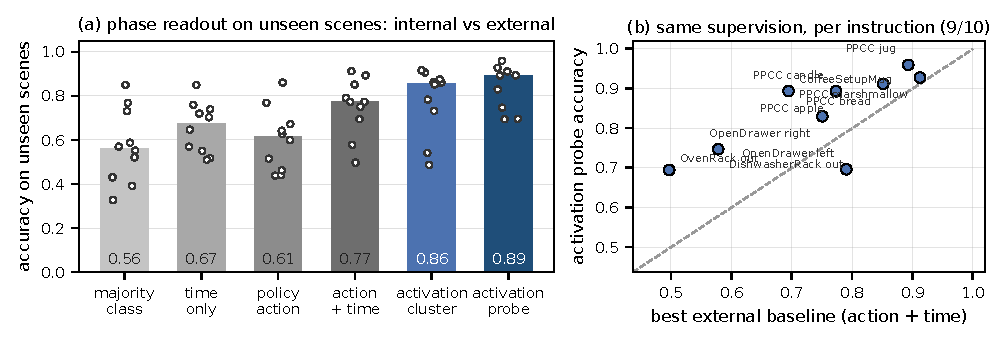
\includegraphics[width=0.96\textwidth]{figs/fig_readout_accuracy.pdf}
  \caption{\new{한 번도 보지 않은 scene에서의 phase 판독 정확도. (a) 방법별 중앙값(점 =
  instruction 10개). activation 기반(파랑)이 시간 대조군·다수 클래스를 크게 앞선다.
  (b) instruction 별 시간 대조군 대 activation 군집 --- 대각선 위가 activation 승(9/10).}}
  \label{fig:readout}
\end{figure*}
\section{결 과}
\new{\textbf{activation 한 스텝만으로 현재 phase를 읽을 수 있다(그림 3).} 한 번도 보지
않은 scene에서 잰 판독 정확도는 비지도 군집 0.86, 지도 probe 0.89(instruction 중앙값)로,
다수 클래스(0.56)와 시간 대조군(0.61)을 크게 웃돈다. macro-F1로 봐도 0.57/0.72 대
0.23/0.29로 같은 격차다. 10개 instruction 중 9개에서 activation이 시간 대조군을 이기며,
격차가 가장 큰 OpenDrawer left는 0.26 대 0.73이다. phase는 대체로 시간 순서대로
진행하므로 ``시계만 봐도 맞힌다''가 가장 강한 반론인데, 실측은 그 반대다. 특히 비지도
군집만으로 0.86이 나온다는 점이 중요하다 --- 구조 자체는 라벨 없이 activation에서 나왔고
라벨은 각 군집에 이름을 붙이는 데만 쓰였다. 군집 중심을 train에서 만들고 평가 스텝은
최근접 배정으로 옮기므로, 재군집화 없이 추론 중 스텝 단위로 그대로 돌릴 수 있다.}

\textbf{발견된 단위는 사람이 정의한 phase보다 잘게 나뉜다\new{(그림 2a).}} 발견된
상태의 평균 구간 길이는 GT phase보다 짧다(k=24에서 4.3 vs 16.1 스텝, 전환율 18.4\% vs
5.0\%; 데이터셋 B에서도 6.0 vs 18.1 스텝). 이 전환은 고정 리듬 아티팩트가 아니고(전환
위치의 주기성 없음), 전환 시점이 GT 경계와 정렬되지도 않는다(z $-$1.0$\sim$+0.5 ---
우연 수준). 그러나 발견 상태를 GT phase 단위로 병합하면 경계 정렬이 유의해진다(z
+1.3$\sim$+4.9). 즉 activation은 GT phase를 그대로 재현하지 않고 그보다 잘게 쪼갠다. \new{이는 군집 수
k를 키운 결과만은 아니다: k를 GT phase 수(3$\sim$6)에 맞춘 k=8에서도 구간 길이는 10개
instruction 전부에서 GT보다 짧고, 에피소드당 전환 수도 상태를 한 번씩만 지나는 상한
(k$-$1=7회)을 모두 넘는다(7.3$\sim$30.0회 = 상태 재방문). 반대로 OvenRack은 같은 k=8에서
GT와 거의 같은 해상도로 병합된다(8.5 vs 8.5 스텝). 다만 이 세분이 의미 있는 하위 구조인지는
본 연구의 범위를 넘으며, 판독 정확도는 세분 여부와 무관하게 성립한다.}

\textbf{각 군집은 특정 단계에 국한된다(그림 1a, 그림 2b).} 한 단계에서 나타난 군집은
다른 단계에서 잘 나타나지 않는다: 군집$\rightarrow$단계 순도 0.80, MI 2.17 bits(상한
2.82), 시간 대조군 margin +1.665 bits. 군집이 최빈 단계 밖에서 나타나는
비율(off-phase rate)의 군집별 중앙값은 instruction 중앙값 0.07이며, 순수한 instruction에서는
0.002까지 내려간다(넓게 걸치는 것도 있어 최대 0.45 --- instruction별 편차가 있다).
데이터셋 B에서도 순도 중앙값은 0.88로 유지된다. phase 하나는 평균 2$\sim$3개 군집으로
세분되어(phase당 군집 수 1.3$\sim$2.7),
대응은 1:1이 아니라 다대일이다 --- 이것이 위의 ``세밀한 하위 분할''과 순도가
공존하는 이유다. 비디오 행동 분절에서 과분할은 통상 벌점이지만, 여기서 세분은
phase-순수한 다대일 대응이며 그 판정 근거는 순도·MI·margin이지 경계 F1이 아니다.

\textbf{단계 정보는 장면 암기로 환원되지 않는다(그림 1b).} 활성화에는 장면(scene)
정보도 섞여 있다(instruction별 mi\_scene 0.02$\sim$0.86 bits). 그러나 instruction 내
scene별 평균을 제거한 잔차에서 scene 정보는 크게 줄어드는 반면(mi\_scene 중앙값
0.44$\rightarrow$0.27 bits) phase margin은 10개 instruction 전부에서 양수로
유지된다(중앙값 +0.34$\rightarrow$+0.31).

\textbf{구조는 모델·데이터를 바꿔도 재현된다.} 같은 데이터에서 구조가 다른 두 압축
모델(AE, SAE)이 같은 스텝에서 전환하고(F1 0.66$\sim$0.75, 무작위 0.51$\sim$0.53, z
+8.8$\sim$+13.5), 독립 재수집 데이터에서 새로 학습해도 같은 성질이 나타난다(seed 간 F1
0.55$\sim$0.58, z +4.3$\sim$+5.1). denoising 슬롯·장면·시드는 에피소드 내 상수라 전환의
원인이 될 수 없다.

\textbf{세밀 단위는 하류 분석에서도 유용하다.} 성공/실패 분리도를 단계 조건부로 잴
때, 발견 상태(instruction별 k=8)가 GT phase보다 높은 분리도를 주는 instruction이 9개 중
4개였다(동급 1, 열세 1; 예: OpenDrawer AUROC 0.93/z4.5 vs GT 0.94/z2.3). 이는 탐색적
관찰이나, 세밀 단위가 사람 정의 단계의 단순 잡음이 아님을 시사한다.



% 지면 여유 시 사용 (해상도-유용성 곡선):
% \begin{figure}[t]
%   \centering
%   
\includegraphics[width=\columnwidth]{figs/fig3_granularity_utility.pdf}
%   \caption{내재적 margin은 k에 단조 증가하지만 하류 성공/실패 층화는 사람 단계
%   수(3~6)보다 촘촘한 k=8에서 최대이다.}
%   \label{fig:utility}
% \end{figure}

\section{한계와 결론}
\new{판독의 근거는 각 스텝을 어느 phase로 볼지에 대한 군집 정체성이지 phase 경계 검출이
아니다 --- 전환 시점 자체는 GT 경계와 정렬되지 않는다(z $\approx$ 0). 또한 GT 라벨 두 벌이
같은 주석 체계의 두 버전이라 ``어떤 phase 정의와도 어긋난다''고는 할 수 없고, 길이 1의 짧은
상태가 구간의 31$\sim$37\%를 차지하는데 그것이 의미 있는 하위 구조인지는 미검증이다.
판독 평가는 scene 단위 held-out이지만 instruction 간 전이는 다루지 않았다.}

\new{결론: VLA의 내부 activation만으로 현재 action phase를 읽을 수 있다 --- 처음 보는
scene에서 정확도 0.86(비지도)/0.89(probe)이며, 시간 정보만 쓰는 대조군(0.61)을 크게
웃돈다. 이 구조는 라벨 없이 얻어지고 scene 성분을 제거해도 유지되며 모델·데이터를 바꿔도
재현된다. 즉 모델이 지금 무슨 작업을 진행 중이라고 표상하는지를 외부 관측 없이 내부에서
스텝 단위로 읽을 수 있으며, 이는 VLA 행동의 설명 신호이자 단계 조건부 개입과 실패 감지의
조건 신호가 된다.}

% \section*{ACKNOWLEDGMENT}
% TODO: 과제 사사 문구

\begin{thebibliography}{9}\footnotesize\setlength{\itemsep}{1pt}
\bibitem{groot} NVIDIA GEAR Team, ``GR00T N1: An Open Foundation Model for
Generalist Humanoid Robots,'' arXiv:2503.14734, 2025.
\bibitem{robocasa} S. Nasiriany et al., ``RoboCasa: Large-Scale Simulation of
Everyday Tasks for Generalist Robots,'' \textit{RSS}, 2024.
\bibitem{saevla} A. Swann et al., ``Sparse Autoencoders Reveal Interpretable and
Steerable Features in VLA Models,'' arXiv:2603.19183, 2026.
\bibitem{observing} H. Buurmeijer et al., ``Observing and Controlling Features in
Vision-Language-Action Models,'' arXiv:2603.05487, 2026.
\bibitem{egsae} X. Jin et al., ``Event-Grounded Sparse Autoencoders for
Vision-Language-Action Policies,'' arXiv:2605.17204, 2026.
\bibitem{mechinterp} B. H\"aon et al., ``Mechanistic Interpretability for Steering
Vision-Language-Action Models,'' \textit{CoRL}, 2025.
\bibitem{safe} Q. Gu et al., ``SAFE: Multitask Failure Detection for
Vision-Language-Action Models,'' \textit{NeurIPS}, 2025.
\bibitem{lotus} W. Wan et al., ``LOTUS: Continual Imitation Learning for Robot
Manipulation Through Unsupervised Skill Discovery,'' \textit{ICRA}, 2024.
\bibitem{options} R. S. Sutton, D. Precup, and S. Singh, ``Between MDPs and
Semi-MDPs: A Framework for Temporal Abstraction in Reinforcement Learning,''
\textit{Artificial Intelligence}, 112:181--211, 1999.
\end{thebibliography}

\end{document}
